\section{Recherche de chemin}
Cette section explique l'infrastructure et la logique qui se trouve derrière la recherche de chemin. Le but est de trouver le chemin le plus court entre deux salles.

\subsection{Nœuds et Graphe}
Afin de pouvoir utiliser un algorithme de recherche de chemin, il faut tout d'abord mettre en place un graphe \cite{wiki-graph}. Un graphe est une structure composée d'un nombre fini de nœuds reliés entre eux. Dans notre cas, chaque nœud est un endroit prédéfini du bâtiment, il existe toujours un chemin entre deux nœuds de ce graphe, voir Figure \ref{fig:pathfinding-nodes}.

\begin{figure}
	\centering
	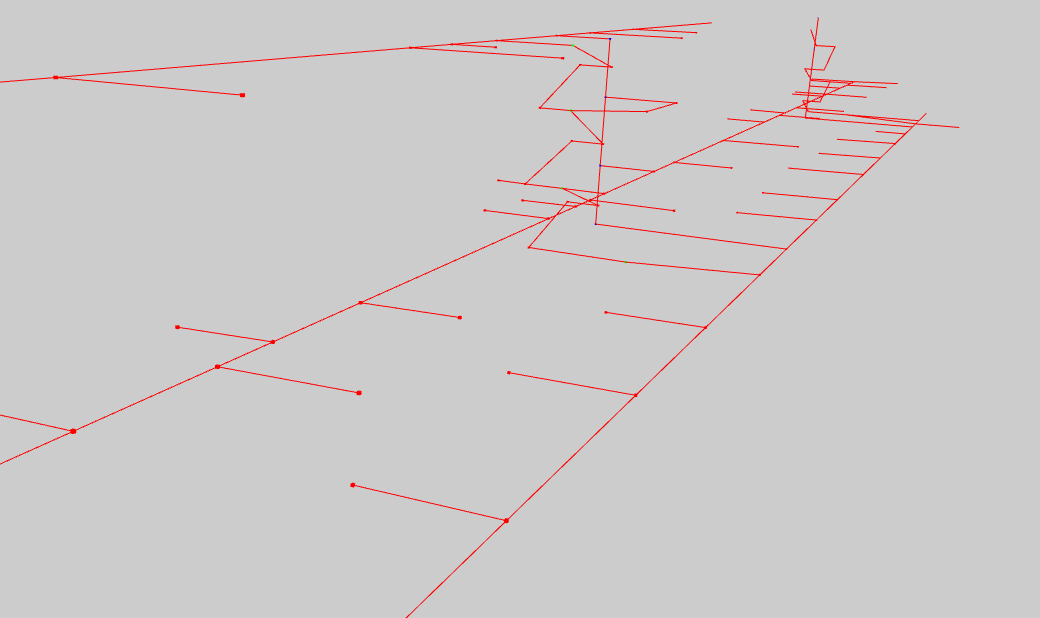
\includegraphics[width=0.9\linewidth]{pathfinding-Nodes}
	\caption{Graphe du bâtiment, les points plus épais sont les nœuds.}
	\label{fig:pathfinding-nodes}
\end{figure}

Un nœud est décrit par les paramètres suivants:
\begin{itemize}[noitemsep]
	\item \emph{id}, nombre, unique;
	\item \emph{nom}, texte, optionnel;
	\item \emph{position}, (x,y,z);
	\item \emph{voisins}, tableau des identifiants voisins.
\end{itemize}

\subsection{Algorithme de recherche de chemin}
Pour privilégier la vitesse de calcul, l'algorithme de recherche de chemin choisi et implémenté est l'algorithme \emph{A*} \cite{wiki-astar} (\textit{A star}). Grâce à ce dernier, on trouve \textit{une des meilleures} solutions en très peu de temps. En utilisant ce dernier sur notre graphe, il est possible de trouver un des meilleurs chemins d'un nœud A à un nœud B.

Ensuite, une nouvelle fonctionnalité est venue s'ajouter au projet. Le but est de trouver les toilettes les plus proches de l'utilisateur. La différence avec la première version est que cette fois on désire chercher une liste de nœuds et plus un seul. Afin d'être sûr de trouver le nœud le plus proche, on ne peut plus utiliser l'algorithme \textit{A*}. C'est pourquoi si on se retrouve dans ce cas là, le programme bascule sur un algorithme de \emph{Dijkstra} \cite{wiki-dijkstra} et avec cette recherche, il suffit de s'arrêter dès que l'on tombe sur un des nœuds que l'on recherchait.